\subsubsection{Package com.sirius.sequenziatore.server.presenter.processowner}
\begin{figure}[H] \centering 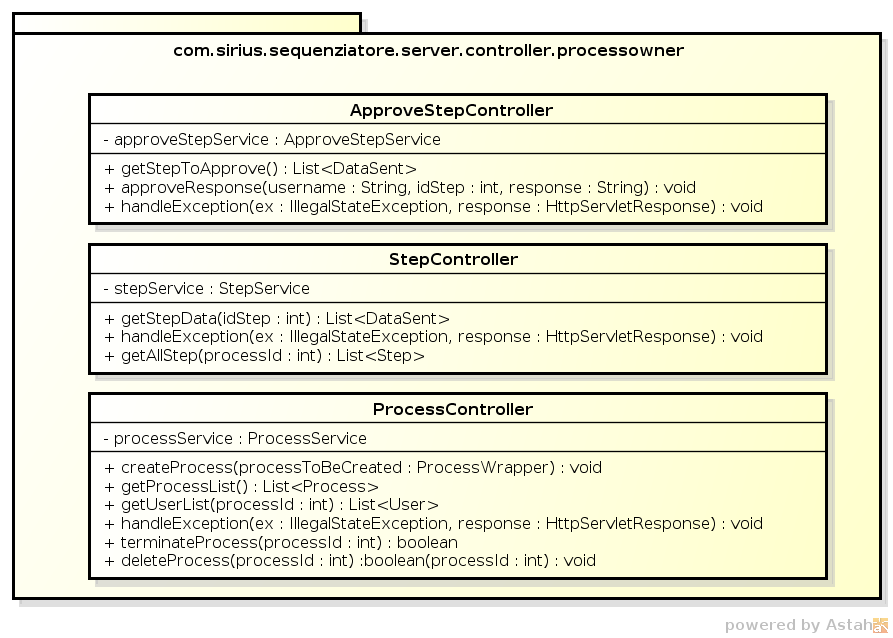
\includegraphics[width=%
\textwidth]
{./classi/server/controllerprocessowner.png} \caption{Diagramma package - \texttt{com.sirius.sequenziatore.server.presenter.processowner}}
\end{figure}
\paragraph{StepController}%----------------------------------------------------------------%
\
\begin{figure}[H] \centering
\includegraphics[trim=0cm 0.8cm 0cm 0cm,clip=true,scale=0.75]%
{./classi/server/stepcontroller.png} \caption{Diagramma classe - \texttt{StepController}}
\end{figure}
\begin{itemize}
	\item \textbf{Descrizione: } Questa classe dovrà fornire al \textit{process owner} tutti i dati inseriti dagli utenti per un dato passo, quindi dovrà restituire una collezione di dati al process owner il quale potrà visionarli;
	\item \textbf{Mappatura base: } \textit{\slash stepdata\slash \{idstep\}\slash processowner}
	\item \textbf{Relazioni con altri componenti: }
	La classe utilizzerà le seguenti classi:
	\begin{itemize}
		\item \texttt{com.sirius.sequenziatore.server.model.DataSent;}
		\item \texttt{com.sirius.sequenziatore.server.model.Step;}
		\item \texttt{com.sirius.sequenziatore.server.service.StepService;}
	\end{itemize}
	\item \textbf{Metodi: }\begin{itemize}
					\item \texttt{+List<DataSent> getStepData(int idStep):}\\
					questo metodo gestisce una richiesta di tipo \textbf{GET} che fornisce al \textit{process owner} tutti i dati inviati dagli utenti per un certo passo dopo averli richiesti al service e in caso di errore lancia un' eccezione;
					\item \texttt{+List<Step> getAllStep(int processId):}\\
					questo metodo riceve una richiesta di tipo \textbf{GET}, e ritorna al process owner una lista contenente tutti i passi di un dato processo, in caso di errore lancia un' eccezione.
					\item \texttt{+void handleException(IllegalStateException,HttpServletResponse response)}:\\
					 questo metodo è un gestore delle eccezioni e sarà incaricato di lanciare al client un errore 422.
				\end{itemize}
\end{itemize}
\paragraph{ProcessController}%----------------------------------------------------------------%
\
\begin{figure}[H] \centering
\includegraphics[trim=0cm 0.8cm 0cm 0cm,clip=true,scale=0.75]%
{./classi/server/processcontroller.png} \caption{Diagramma classe - \texttt{ProcessController}}
\end{figure}
\begin{itemize}
	\item \textbf{Descrizione: } Questa classe permetterà la creazione di un processo da parte del \textit{process owner} e sarà adibita a fornire la lista di tutti i processi esistenti nel sistema;
	\item \textbf{Mappatura base: } \textit{\slash process\slash processowner}
	\item \textbf{Relazioni con altri componenti: }
	La classe utilizzerà le seguenti classi:
	\begin{itemize}
		\item \texttt{com.sirius.sequenziatore.server.model.Process;}
		\item \texttt{com.sirius.sequenziatore.server.model.User;}
		\item \texttt{com.sirius.sequenziatore.server.service.ProcessService;}
		\item \texttt{com.sirius.sequenziatore.server.controller.utilities.ProcessWrapper;}
	\end{itemize}
	\item \textbf{Metodi: }
				\begin{itemize}
					\item \texttt{+void createProcess(Process processToBeCreated):}\\
					questo metodo gestisce una richiesta di tipo \textbf{POST} e incarica il service dell' inserimento del nuovo processo nel database, in caso di errori lancia un' eccezione;
					\item \texttt{+List<Process> getProcessList():}\\
					 questo metodo gestisce una richiesta di tipo \textbf{GET} e restituisce al \textit{process owner} una lista di processi che può visualizzare o in caso di errori lancia un' eccezione;
					 \item \texttt{+List<User> getUserList(int processId):}\\
					 metodo che riceve una richiesta di tipo \textbf{GET} da parte del process owner e restituisce una lista contenente tutto gli utenti che stanno eseguendo un processo.
					 \item \texttt{+boolean terminateProcess(int processId):}\\
					 metodo che gestisce una richiesta di tipo \textbf{POST} e che affida al service l' incarico di terminare il processo, in caso di errore lancia un' eccezione.
					 \item \texttt{+boolean deleteProcess(int processId):}\\
					 metodo che gestisce una richiesta di tipo \textbf{POST} e che affida al service l' incarico di eliminare il processo, in caso di errore lancia un' eccezione.
					  \item \texttt{+void handleException(IllegalStateException,HttpServletResponse response)}:\\
					 questo metodo è un gestore delle eccezioni e sarà incaricato di lanciare al client un errore 500.
				\end{itemize}
\end{itemize}
\paragraph{ApproveStepController}%----------------------------------------------------------------%
\
\begin{figure}[H] \centering
\includegraphics[trim=0cm 0.8cm 0cm 0cm,clip=true,scale=0.75]%
{./classi/server/approvestepcontroller.png} \caption{Diagramma classe - \texttt{ApproveStepController}}
\end{figure}
\begin{itemize}
	\item \textbf{Descrizione: } Questa classe serve per fornire al \textit{process owner} i dati da approvare e per gestire quali passi siano stati approvati quali no, qualora un passo non venga approvato, verrà rimosso dal \textit{database};
	\item \textbf{Mappatura base: } \textit{\slash approvedata}
	\item \textbf{Relazioni con altri componenti: }
	La classe utilizzerà le seguenti classi:
	\begin{itemize}
		\item \texttt{com.sirius.sequenziatore.server.model.DataSent;}
		\item \texttt{com.sirius.sequenziatore.server.service.ApproveStepService;}
	\end{itemize}
	\item \textbf{Metodi: }\begin{itemize}
					\item \texttt{+List<DataSent> getStepToApprove():}\\
					 il metodo gestisce una richiesta di tipo \textit{GET}, e restituirà un oggetto di tipo List<DataSent> contenente tutti i dati che richiedono approvazione, in caso di errore lancia un' eccezione;
					\item \texttt{+void approveResponse(String username,int idStep,String response):}\\
					il metodo gestisce una richiesta di tipo \textit{POST}, riceve i dati di un passo che ha subito la moderazione del \textit{process owner} e ne affida al service l' elaborazione, in caso di errore lancia un' eccezione;
					\item \texttt{+void handleException(IllegalStateException,HttpServletResponse response)}:\\
					 questo metodo è un gestore delle eccezioni e sarà incaricato di lanciare al client un errore 422.
				\end{itemize}
\end{itemize}